\documentclass[a4paper, UKenglish, 11pt]{uiomaster}
\usepackage{lipsum}
\usepackage[subpreambles=true]{standalone}

% Explain EEG
% Explain how EEG sources can be modeled/simulated (include the first attempt done in 1949)
% Head models (New York Head Model)

\begin{document}
\chapter{Results}
As mentioned in chapter 1, an important topic in EEG signal analysis is the inverse problem of going from measured EEG signals to localized equivalent current dipoles, so-called source localization. In this chapter we will be training and presenting two different(?) neural networks used to localize single dipole sources in the human cortex. Section ...  and ... deal with training a simple feed forward neural network and presenting its results.


\section{The dataset}
The cortex matrix of the New York Head Model (NYHM) consists of 74382 points, which refer to the number of possible positions for localization of a dipole source. When training the FFNN we will be using a data set consisting of simulated EEG signals corresponding to dipol sources with randomly selected positions within the cortex matrix. The final data set consists of 10 000 rows, where each row corresponds to one sample, or let us say - one patient. Within the data set we have 231 columns, also referred to as features, representing the dipole measure at every EEG electrode. Thus, we are left with a design matrix with size 10 000 x 231.

In order to train the network faster, one commonly split the data set into mini-batches, which is also done here. When splitting the data such a way, the weights of connection between neurons are updated after each propagation, making the network converge considerable faster. There might be Through trial and error we landed on a batch size equal to 30.

% Scaling
% Every potential distribution presented to the network is first average referenced by subtracting the average of all potential values. Subsequently, the average referenced potentials are normalized by dividing them by the magnitude of the largest. The dipole location parameters are normalized to 1 with respect to the radius of the outer head boundary in the spherical head model (9.2 cm). In the case of a realistically shaped head model, the location parameters are normalized with respect to the radius of the best-fitting sphere for the scalp–air interface.

% As was pointed out in the previous section, the optimal dipole orientation (in the leastsquares sense) for a given location can be calculated in a straightforward manner. Therefore, we will use neural networks to estimate only the dipole location parameters.
\section{Easy example}

\begin{figure}[!htb]
    \centering
    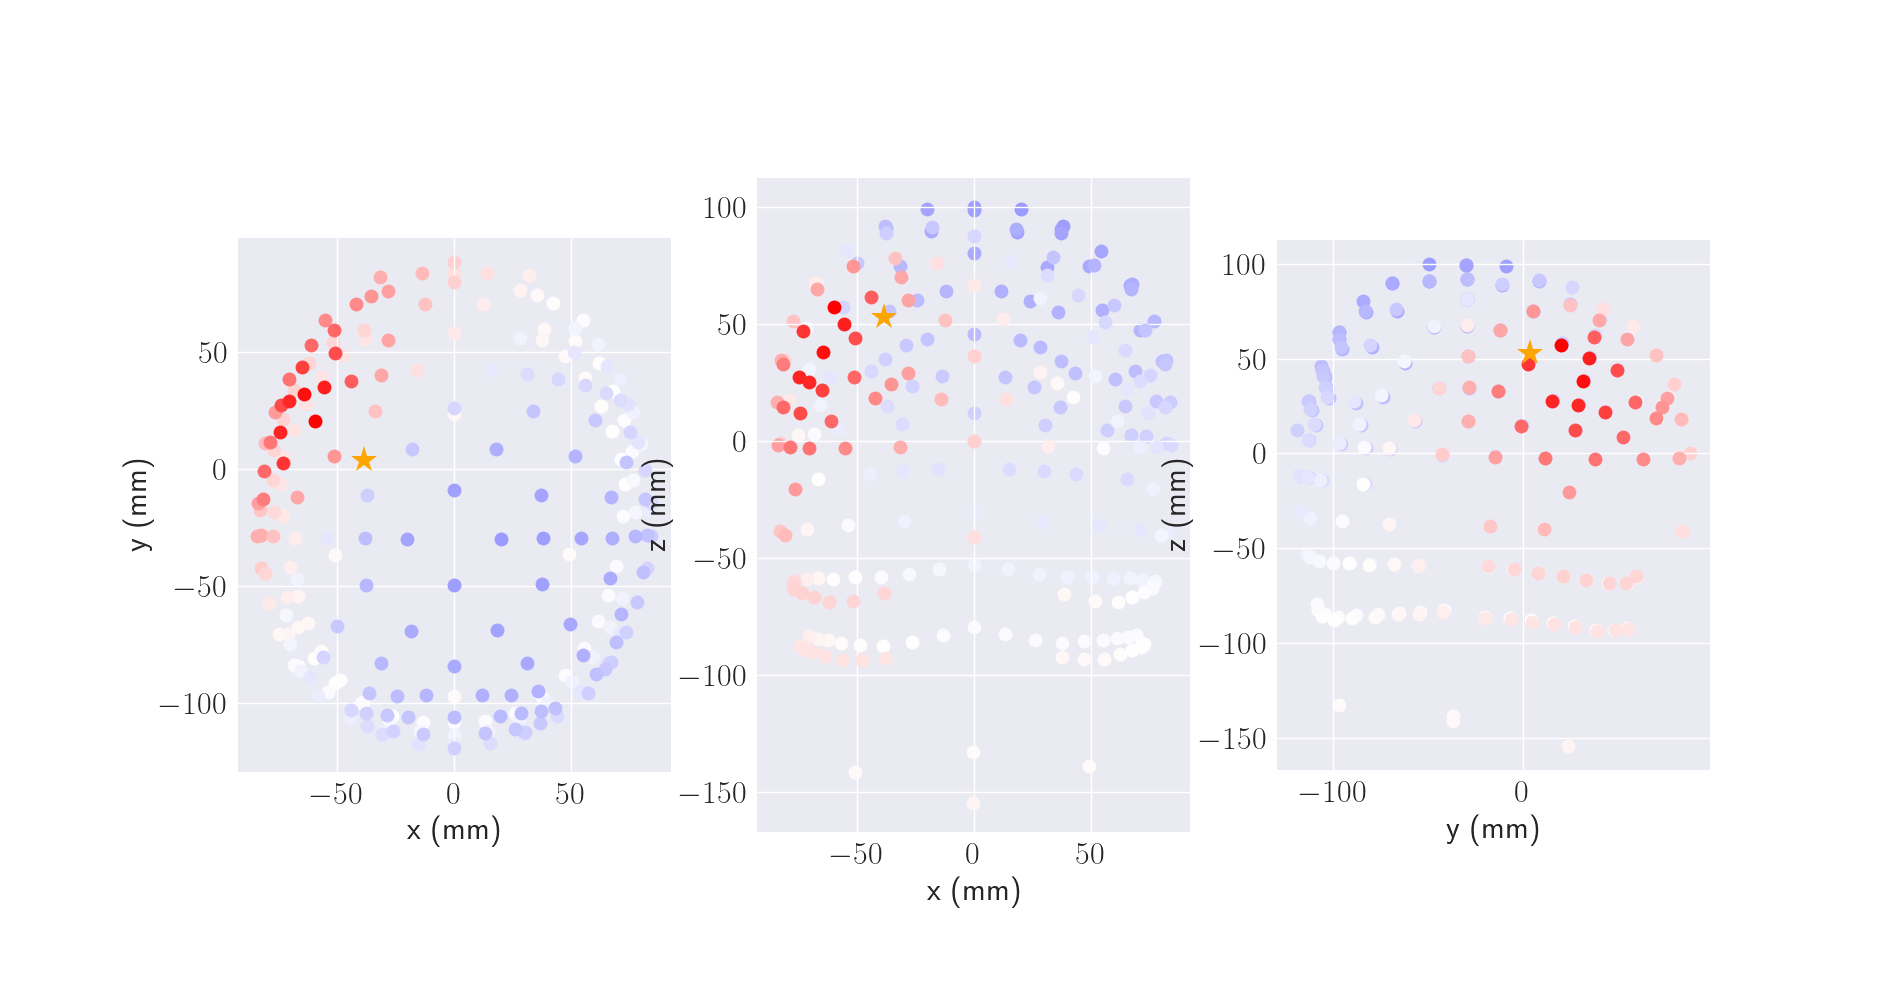
\includegraphics[width=\linewidth]{../Code/plots/finals/eeg_field_1_1.png}
    \caption{Example 1 dipole. }
    \label{fig:eeg_field_1_dipole_example}
\end{figure}

\begin{figure}[!htb]
    \centering
    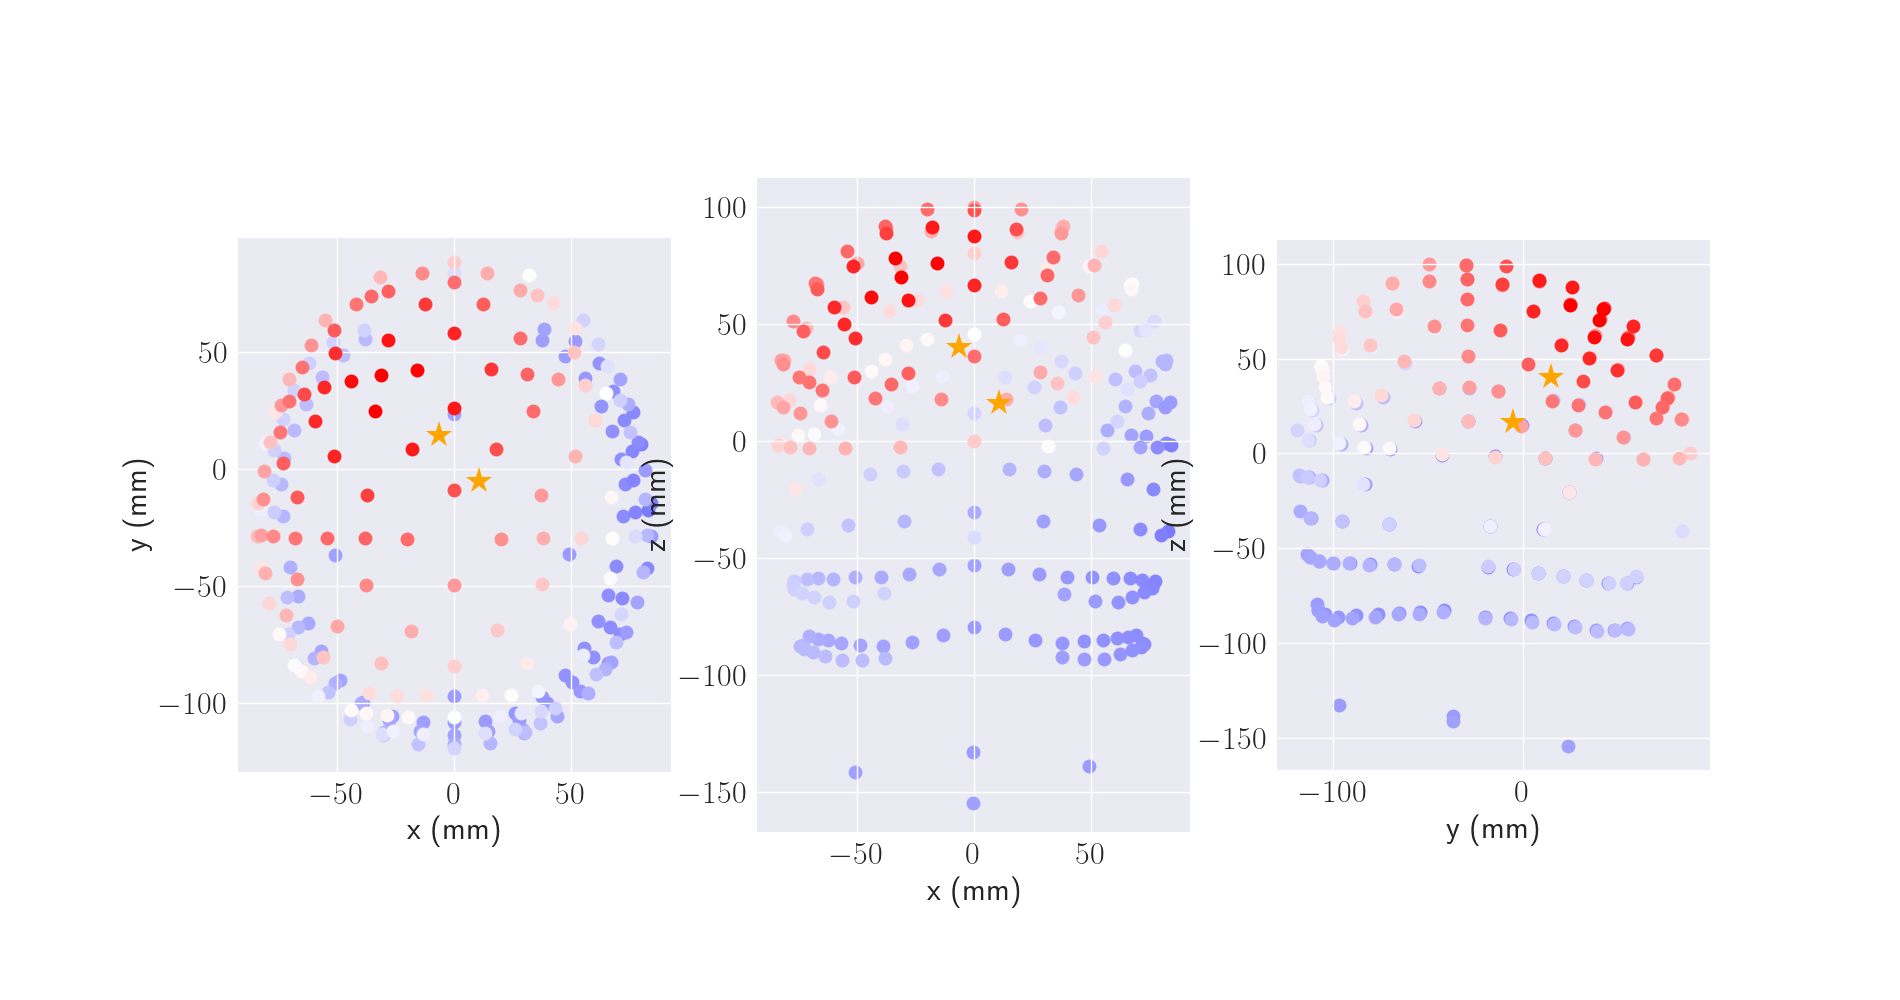
\includegraphics[width=\linewidth]{../Code/plots/finals/eeg_field_2_2.png}
    \caption{Example 2 dipoles. }
    \label{fig:eeg_field_2_dipole_example}
\end{figure}

\section{Feed-Forward Neural Network Approach for localizing single dipole sources}
The feedforward neural network (FFNN) was one of the first artificial neural network to be adopted and is yet today an important algorithm used in machine learning. The feed forward neural network is the simplest form of neural network, as information is only processed forward, from the input nodes, through the hidden nodes and to the output nodes.

The FFNN that are trained to solve the inverse problem of ours has an input layer of 231 neurons, corresponding to the M = 231 electrode measures of the potentials. The input layer is followed by three hidden layers with 120, 84 and 16 hidden neurons, respectively. The final output layer holds the predicted x-, y- and z- position of the desired dipole source. For the neurons of the input layers we use the linear activation function ReLu, while for the neurons of the hidden and output layers, we chose the much used hyperbolic tangent activation function.

Cost function

\subsection{Training, testing and evaluation}
In order to make an ANN that generalizes well to new data we split our data into training and testing sets. Randomly selecting 80 percent of the rows in the full dataset, we put this into a separate one and call it our training set. The remaining 20 percent is put into the test set. In practice, the training data set consists of pairs of an input vector with EEG signals and the corresponding output vector, where the answer key is the x-, y- and z coordinate of the dipole source. The neural network is then feed with the training data and produces an estimation of the localization of the dipole. The estimation is found by the network through optimizing the parameters $\beta$ minimizing the cost function, or said in other words, through finding parameters for the function that produces the smallest outcomes, meaning the smallest errors. The result provided by the network is then compared with the target, for each input vector in the training data. Adjustment of parameters...

When the network is fully trained, we have a final model fit on the training data set. Feeding the network with the test data set, we can assess the performance of the network. The predictions of the fully trained network can now be compared to the holdout data's true values to determine the model's accuracy.

In figure \ref{fig:single_dipole_accuracy_FFNN} we have provided the bias-variance trade-off for when using Tanh as activation function. We notice that error of the model is approaching 0 and that the variance between the two curves decreases for an increasing number of epochs.


\begin{figure}[!htb]
    \centering
    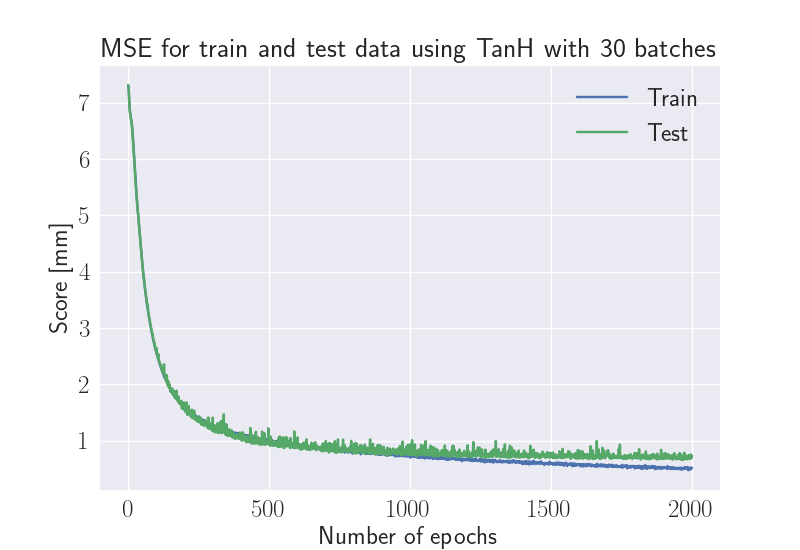
\includegraphics[width=\linewidth]{../Code/plots/finals/MSE_**multiple_dipoles_1_noise10_TanH_30_2000.png}
    \caption{The validation accuracy for simple Feed Forward Neural Network with 10 000 samples with tanh activation function. }
    \label{fig:single_dipole_accuracy}
\end{figure}

% \begin{figure}[!htb]
%     \centering
%     \includegraphics[width=\linewidth]{../Code/plots/NN/MSE_NN_noise_TanH_100_3000.png}
%     \caption{The validation accuracy for simple Feed Forward Neural Network with 10 000 samples with tanh activation function and 10$\%$ noise added to the data. }
%     \label{fig:single_dipole_accuracy}
% \end{figure}

\begin{figure}[!htb]
    \centering
    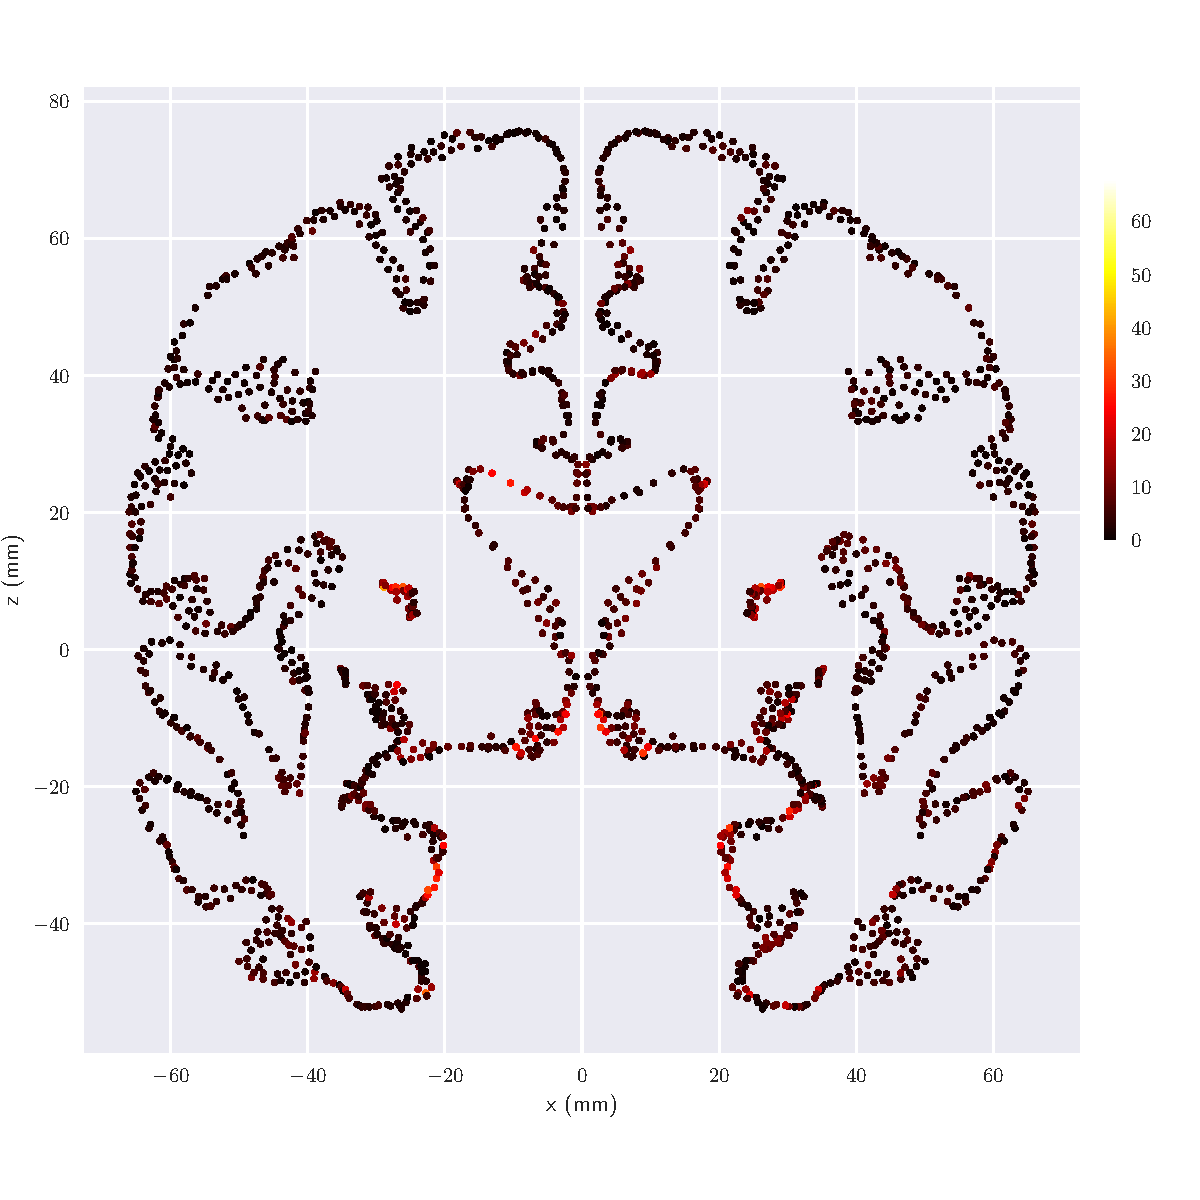
\includegraphics[width=\linewidth]{../Code/plots/finals/mse_y_plane.pdf}
    \caption{The mean squared error of the location accuracy (NN) at different dipole locations
    in the y cross section.}
    \label{fig:single_dipole_accuracy}
\end{figure}



\section{Convolution Neural Network Approach for localizing single dipole sources}

Some results for the prediction of location for single current dipoles.


\begin{figure}[!htb]
\centering
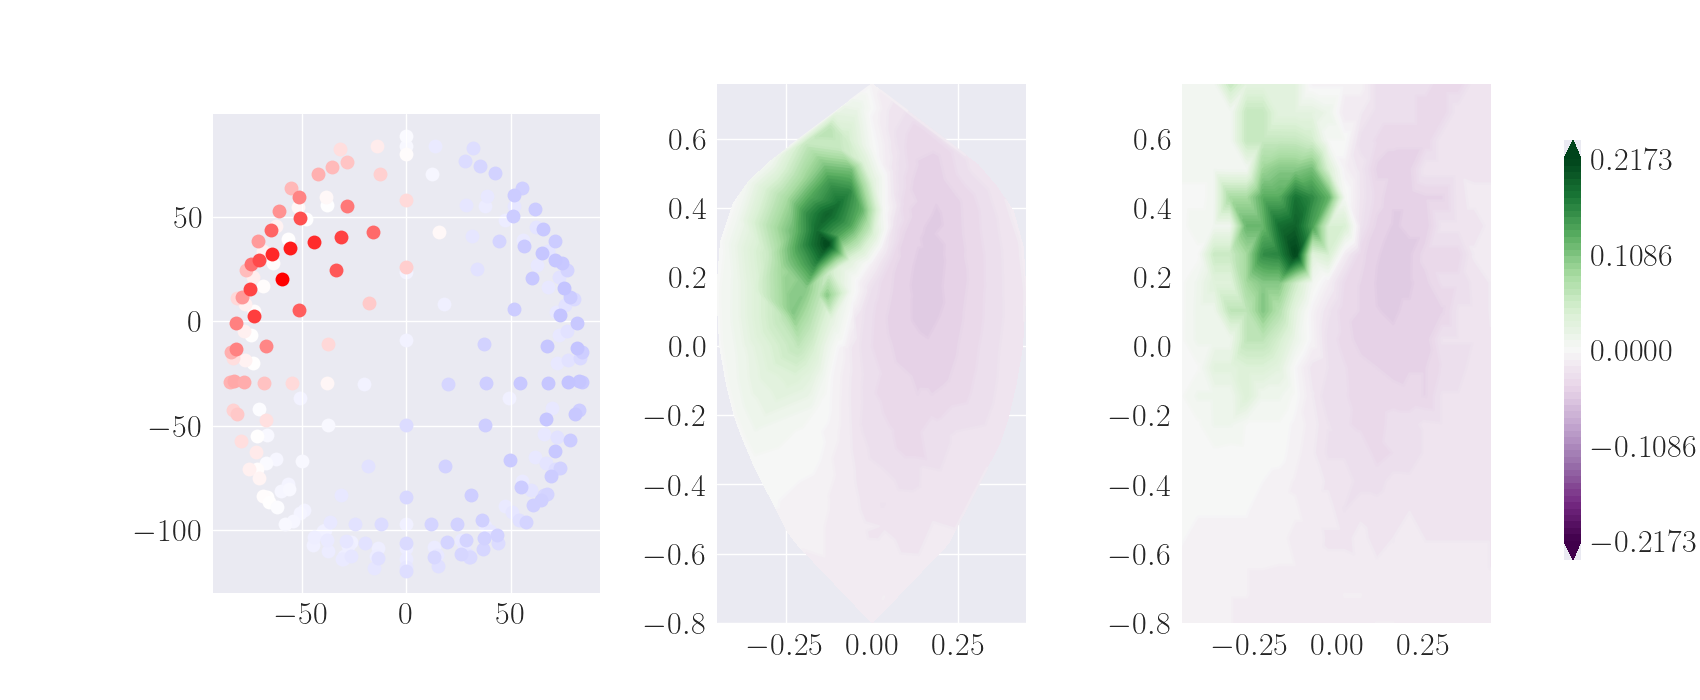
\includegraphics[width=\linewidth]{../Code/plots/finals/new_eeg_dipole_pos_0.png}
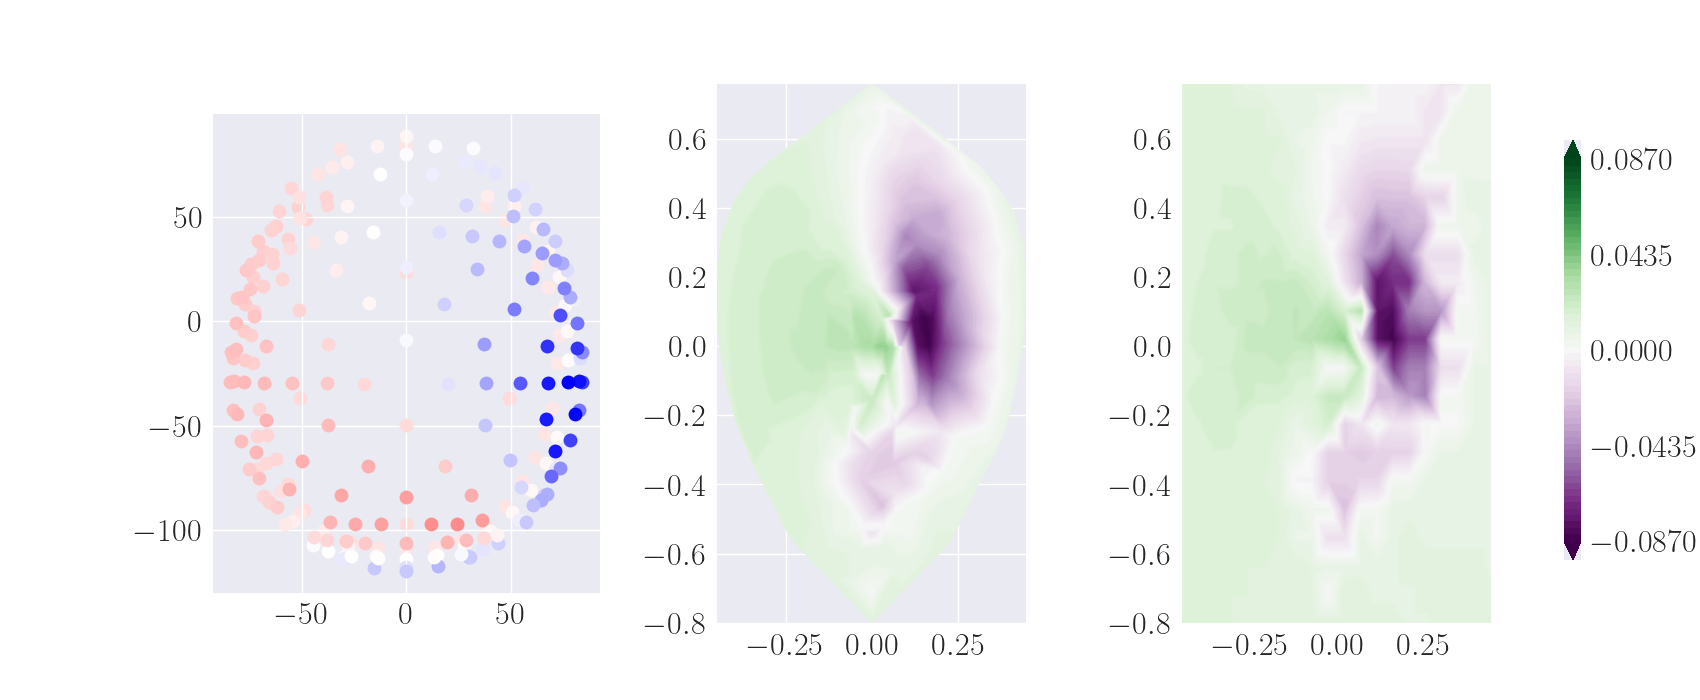
\includegraphics[width=\linewidth]{../Code/plots/finals/new_eeg_dipole_pos_4.png}
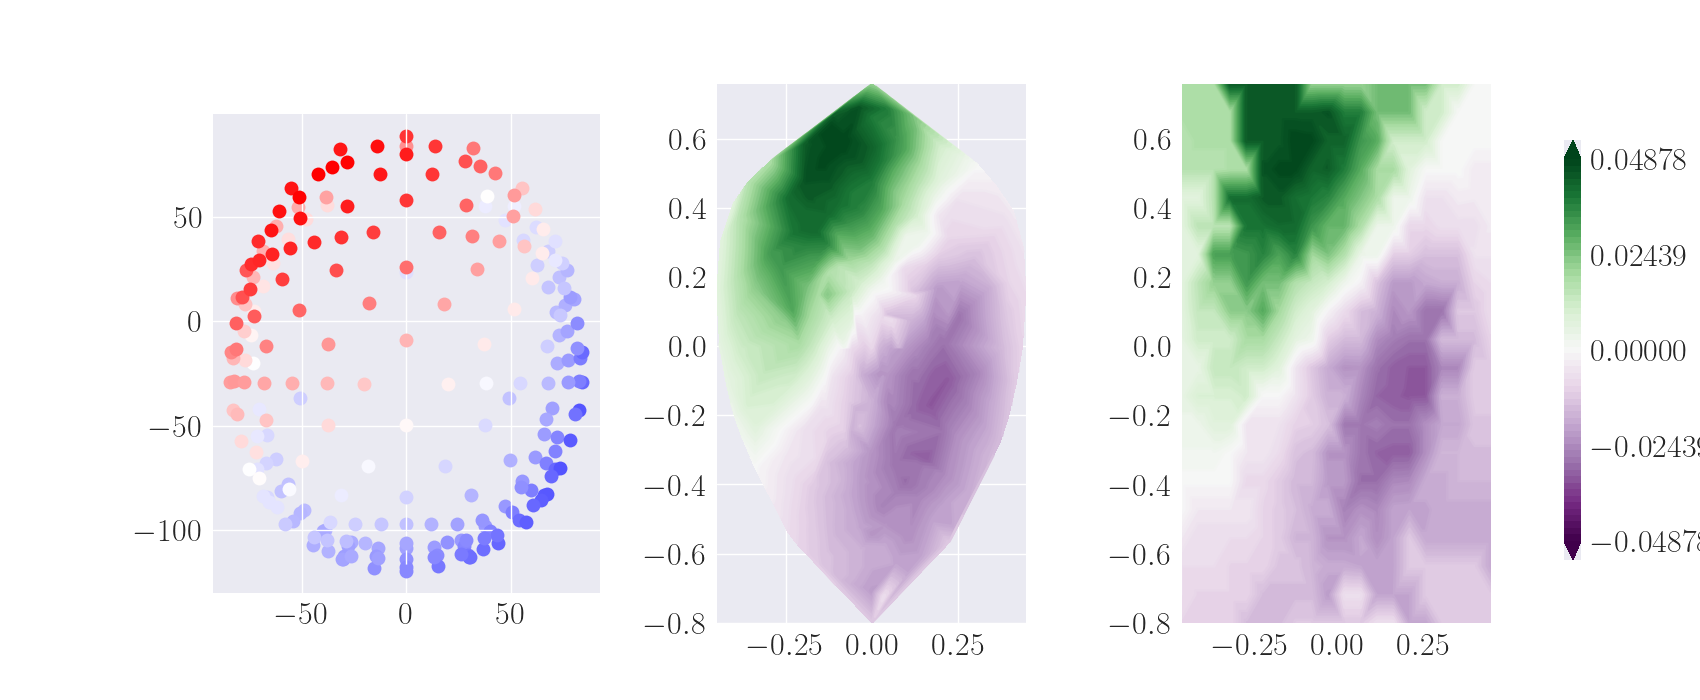
\includegraphics[width=\linewidth]{../Code/plots/finals/new_eeg_dipole_pos_6.png}

\caption{\newline
\textbf{Right}: EEG measure for 3 different samples measured in $\mu V$. \newline
\textbf{Middle and Left}: Illustration of the interpolation of the EEG data into two-dimensional matrix.}
\label{fig:eeg_dipole_pos_0}

\end{figure}

\begin{figure}[!htb]
    \centering
    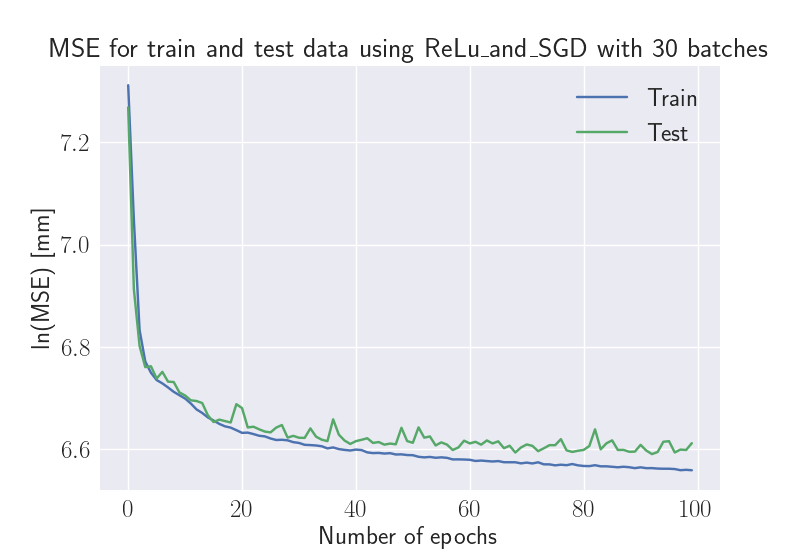
\includegraphics[width=\linewidth]{../Code/plots/finals/MSE_CNN_dipoles_2_interpolated_CNN_20x20_10000_ReLu_and_SGD_30_100.png}
    \caption{The validation accuracy for Convolutional Neural Network with 10 000 samples (20x20 matrix) with ReLU activation function. }
    \label{fig:single_dipole_accuracy_CNN_2d}
\end{figure}

% \begin{figure}[!htb]
%     \centering
%     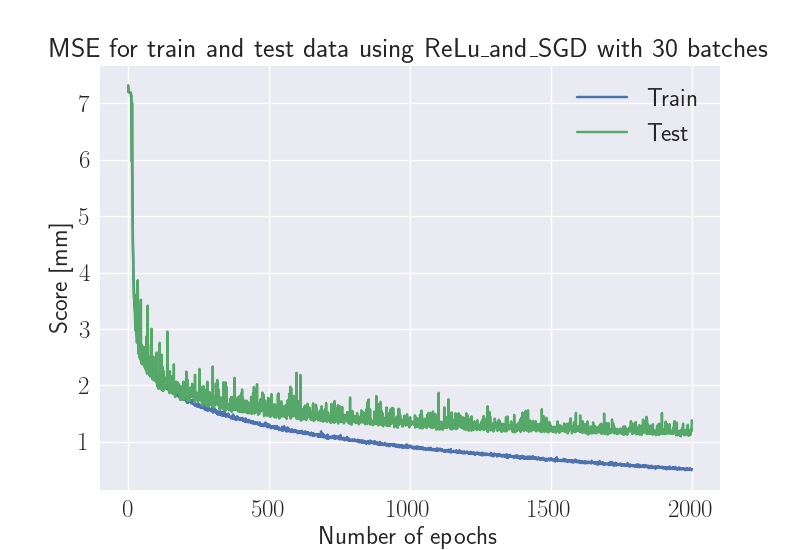
\includegraphics[width=\linewidth]{../Code/plots/CNN/MSE_interpolated_CNN_20x20_10000_ReLu_and_SGD_30_2000.png}
%     \caption{The validation accuracy for Convolutional Neural Network with 10 000 samples (20x20 interpolated matrix) with ReLU activation function. }
%     \label{fig:single_dipole_accuracy_CNN}
% \end{figure}


\section{Region of Active Correlated Current Dipoles}

Some results for the prediction of the size and location of current dipole populations.

\begin{figure}[!htb]
    \centering
    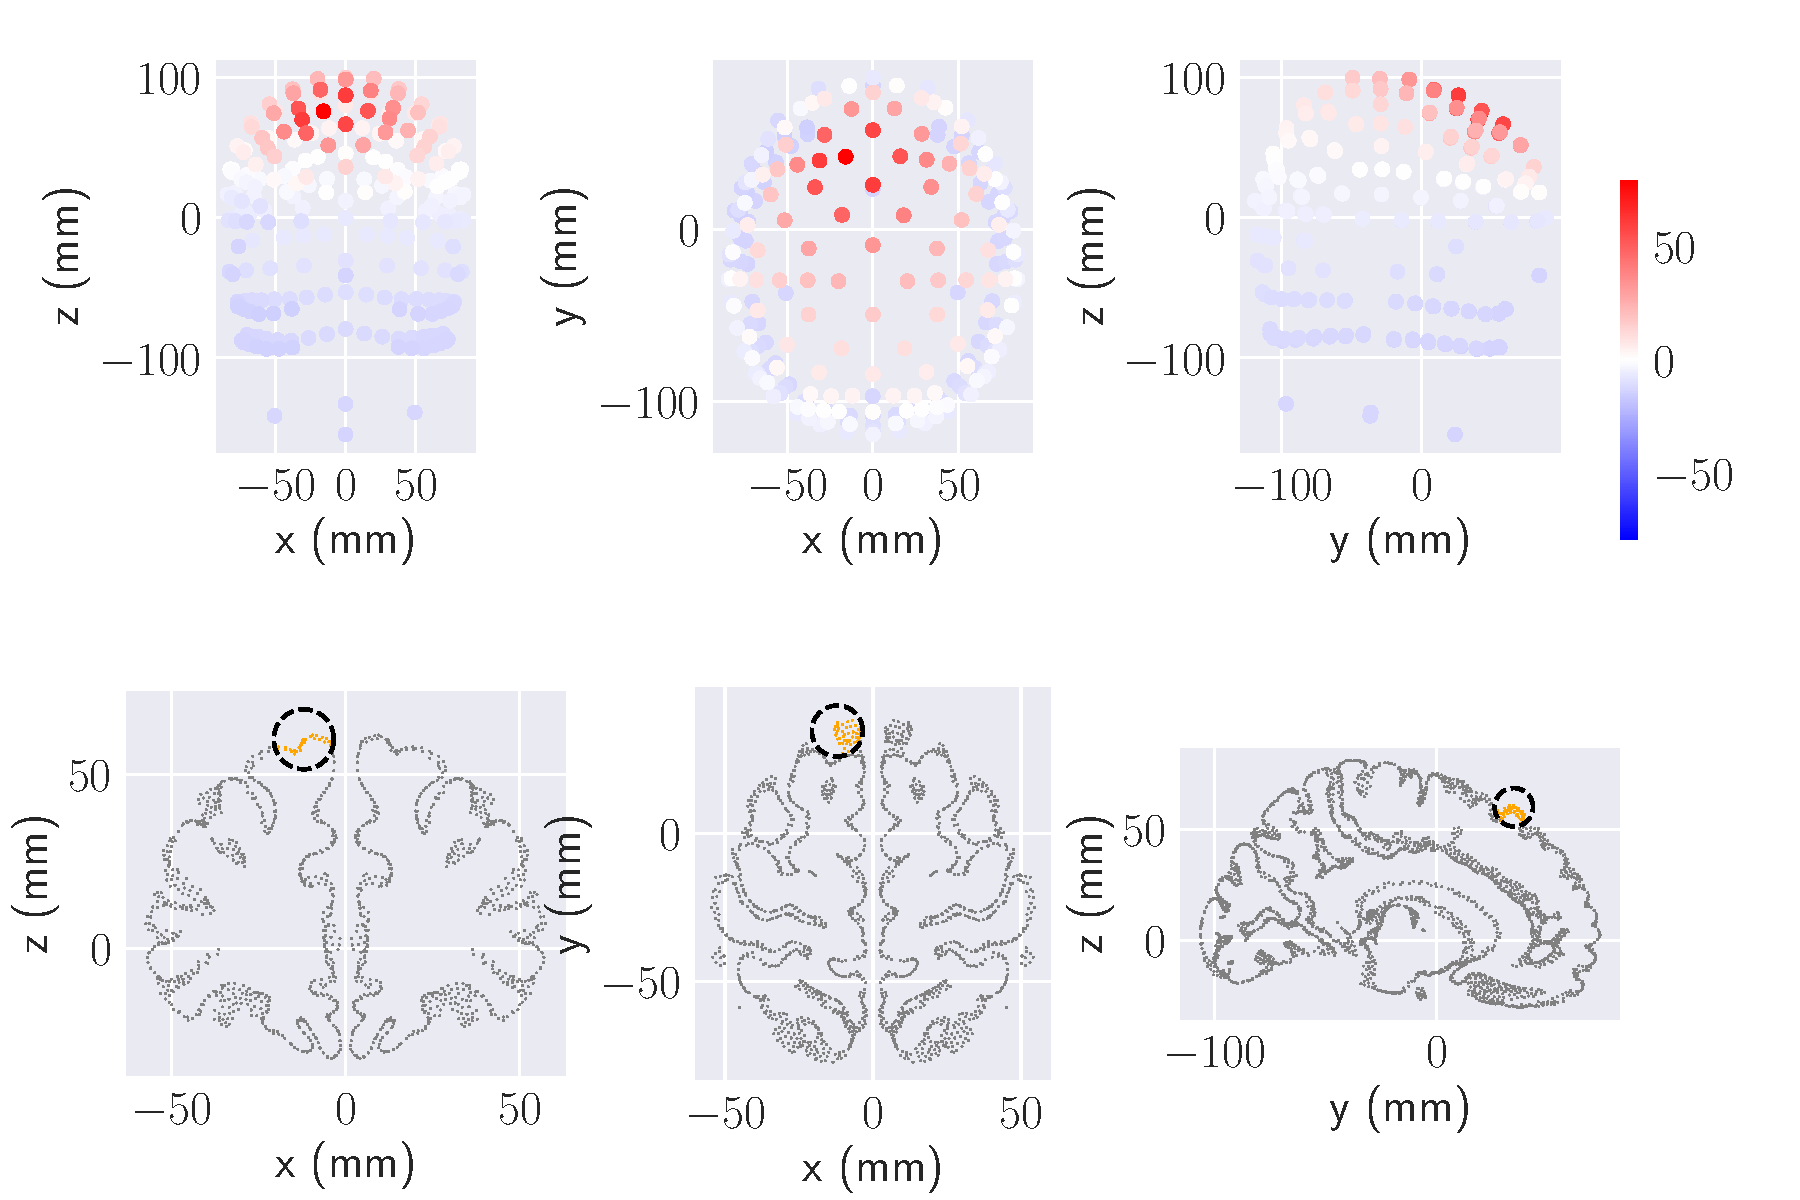
\includegraphics[width=\linewidth]{../Code/plots/finals/new_dipole_area_reduced_0.pdf}
    \caption{New text.}
    \label{fig:dipole_area}
\end{figure}

\begin{figure}[!htb]
    \centering
    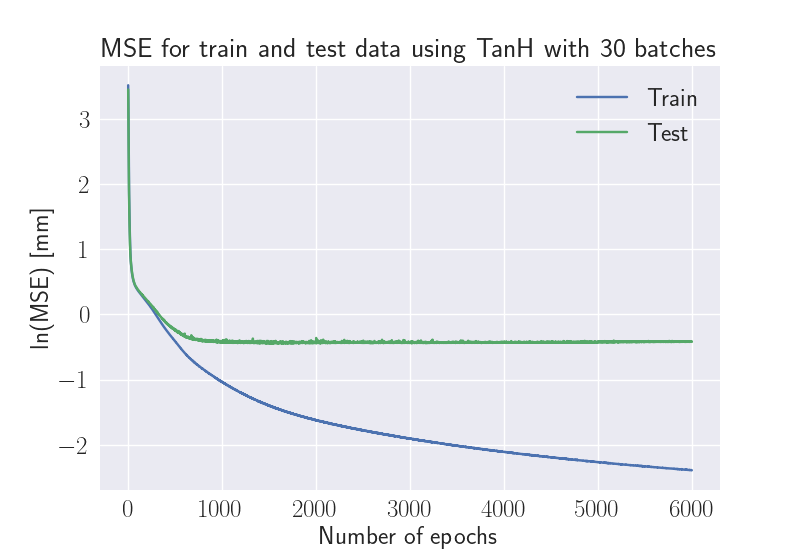
\includegraphics[width=\linewidth]{../Code/plots/finals/MSE_NN_1_10000_l1_l2_20mm_TanH_30_6000.png}
    \caption{New text.}
    \label{fig:dipole_area_result}
\end{figure}

\end{document}